\section{模型准备}
\subsection{WLAN工作流程}

在 AP 或 STA 端,发送和接收数据信号的功能不能同时进行。根据题目要求,本文遵循的端口发送数据和接收信号的流程,如下图所示。

% TODO: \usepackage{graphicx} required
\begin{figure}[H]
	\centering
	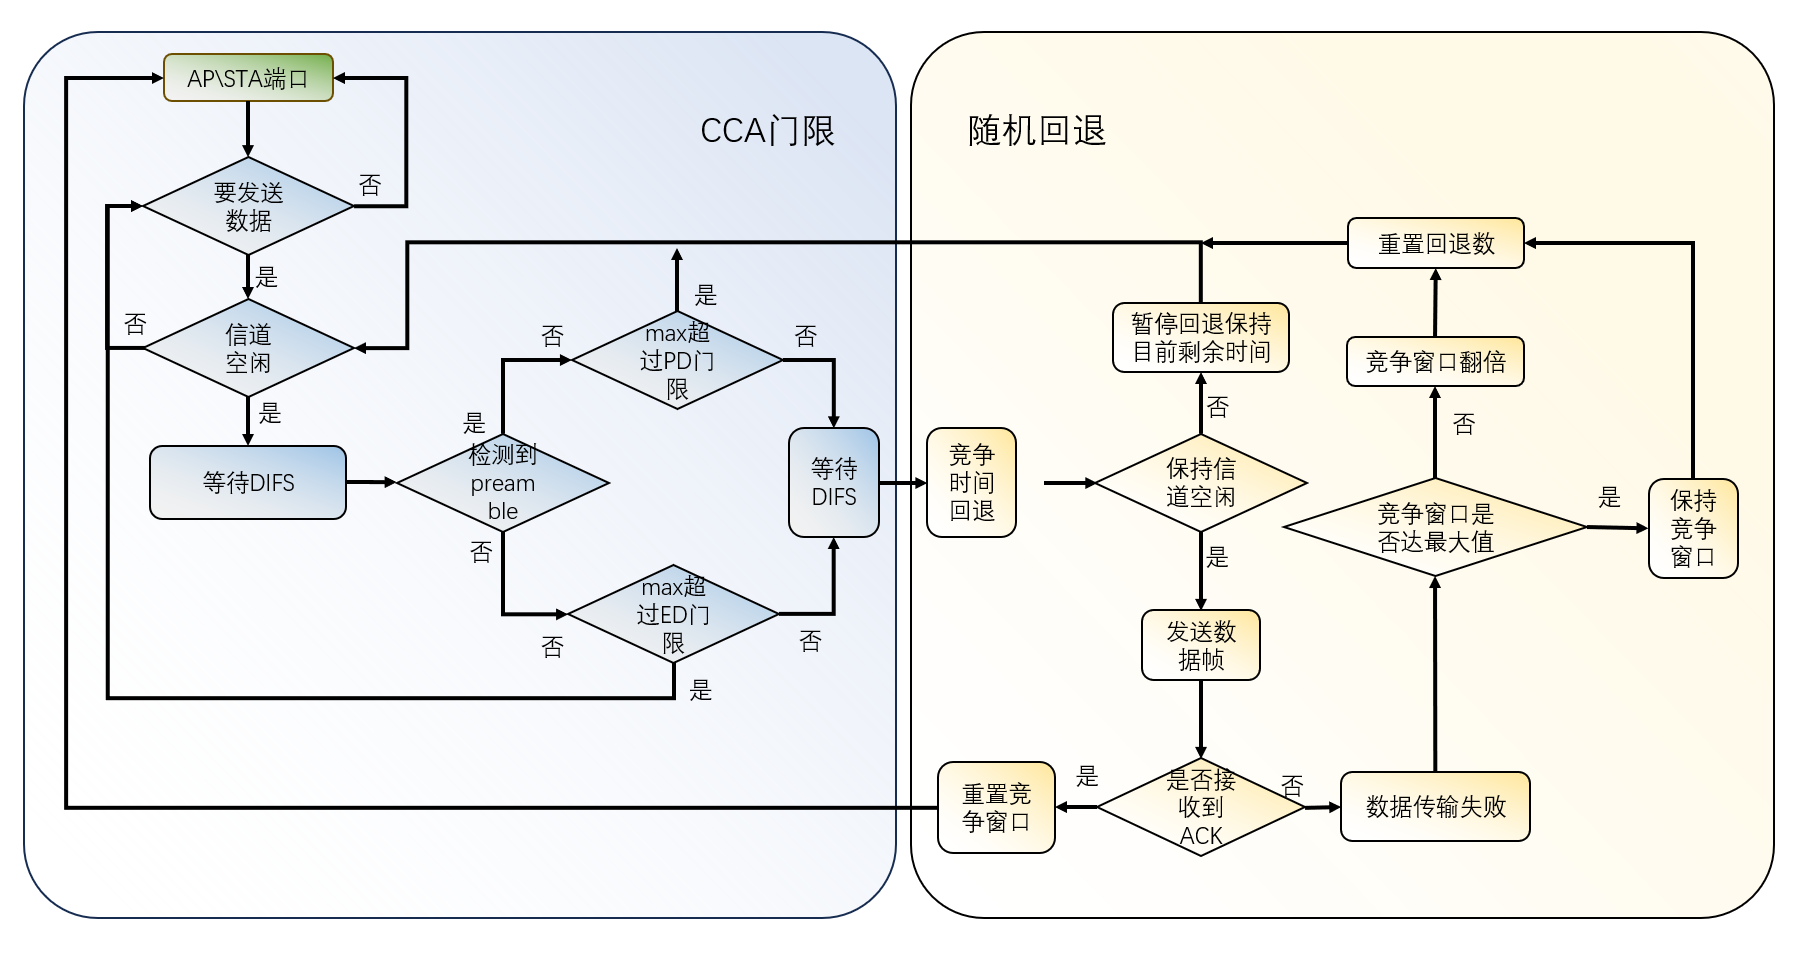
\includegraphics[width=0.9\linewidth]{figures/4.1}
	\caption{端口发送数据流程图}
	\label{fig:端口发送数据流程图}
\end{figure}

图4.1展示了 AP(接入点)在发送数据帧时遵循的基本步骤。此过程涉及 802.11 标准中的竞争窗口(CW)和退避机制,以确保多设备共享同一信道时避免冲突。步骤如下:

\begin{itemize}
	\item 检查是否要发送数据:如果AP有数据需要发送,则进入下一步。
	\item 确保信道空闲:即基于是否处于nav时段确认信道空闲与否或者其他方式确认信道空闲。
	\item 等待 DIFS 时间:AP 等待指定的时间间隔DIFS以确认信道空闲。
	\item 检测 preamble:通过是否错过preambel头选择使PD门限还ED门限判定信道空闲。
	\item 判定PD门限:如果检测到了preamble头,则选择PD门限判定信道空闲,噪声RSSImax超PD门限,说明信道繁忙,返回等待信道空闲。
	\item 判定ED门限:如果未检测到preamble头,则使用ED门限,如果检测到的RSSImax超PD门限),说明信道繁忙,返回等待信道空闲。
	\item 竞争时间回退:如果信道空闲满足发送条件,AP 将从竞争窗口CW随机选择一个竞争时间。如果在此期间信道保持空闲,AP 将发送 RTS 或 CTS 数据帧,来获取信道使用权。
	\item 暂停回退:如果收到 CTS,AP 暂停回退计数器并保持当前剩余时间。
	\item 发送数据帧:如果信道保持空闲且回退时间到0,AP 发送数据帧。
	\item 接收到 ACK:如果成功发送数据帧并接收到确认帧(ACK),则结束发送过程。
	\item 竞争窗口翻倍:发送结束等待超时,长时间未受到ACK确认帧,则会使得CW增大,即在窗口未达到CWmax情况下CW翻倍,重新进行随机回退机制。
\end{itemize}

综上,该流程图展示了 CSMA/CA(载波监听多路访问/冲突避免)协议在无线局域网中的运作,以防止数据帧冲突。当信道繁忙时,设备会退避一段时间后再尝试发送,而在发生冲突时,设备会增大竞争窗口,减少再次冲突的可能性。

% TODO: \usepackage{graphicx} required
\begin{figure}[H]
	\centering
	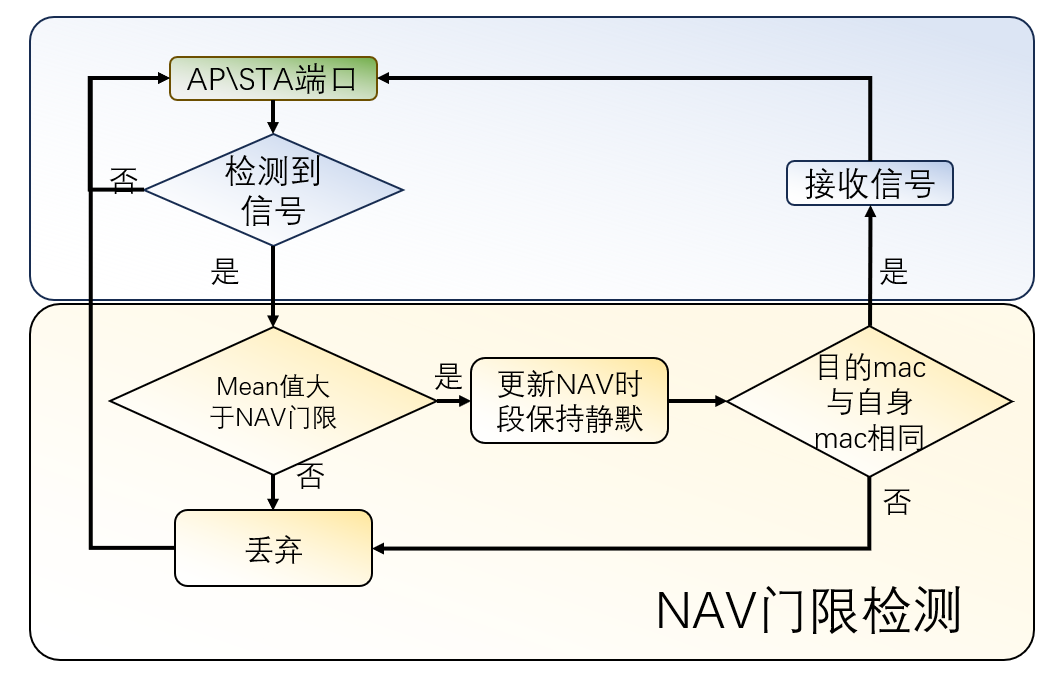
\includegraphics[width=0.7\linewidth]{figures/4.2}
	\caption{端口接收数据流程图}
	\label{fig:端口接收数据流程图}
\end{figure}

图4.2展示了一个简单的无线设备(如AP或STA)在接收信号时的过程。在这个过程中,设备首先判断是否有信号到达,然后根据信号的情况决定是否接收或丢弃信号。具体步骤如下:

\begin{itemize}
	\item AP/STA端口:设备从端口获取信号。
	\item 检测信号:设备检查是否有信号输入。
	\item Mean值与NAV门限比较:若检测到信号,计算其平均值(Mean值)并与NAV门限比较。若Mean值小于或等于NAV门限,设备将忽略该信号。
	\item 更新NAV时段:若Mean值大于NAV门限,设备更新NAV时段,并保持静默状态,停止发送数据以便其他设备发送。
	\item 接收信号:如果Mean值大于NAV门限,设备继续接收信号。
	\item 目的MAC地址匹配:检查信号的目的MAC地址是否与自身相同。若相同,继续处理该信号;若不同,设备将丢弃该信号。
\end{itemize}

综上,本文简化了无线设备在接收信号时的行为,主要关注信号的质量和目的地址的匹配。


\subsection{训练集参数分析}

在了解并对无线设备的发送与接收信号行为流程后,如果预要利用好数据,需要对应题目给出的信息进行训练集中特征的分析,对不同的参数信息有一定的了解,尤其重点关注在题干中出现的信息类别中的数据。


\begin{figure}[H]
	\centering
	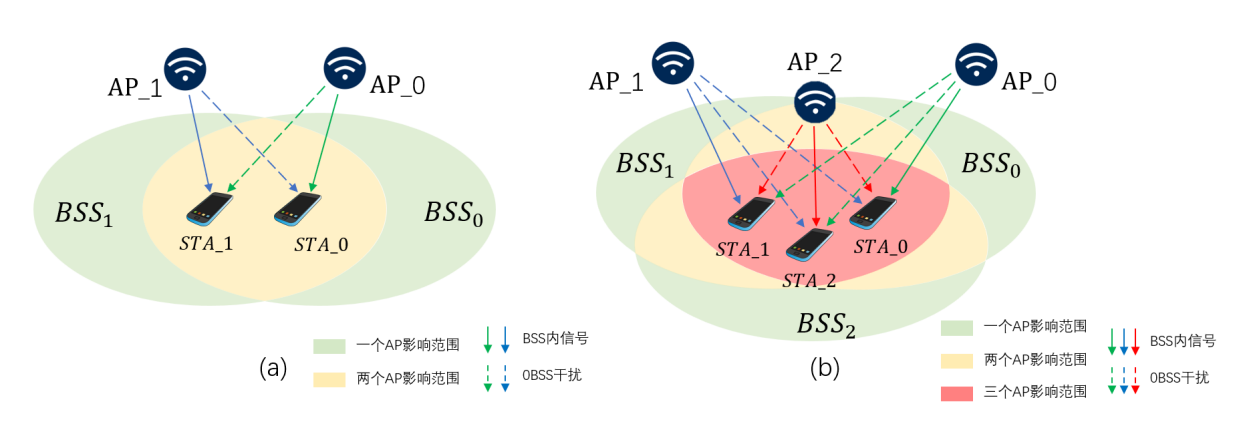
\includegraphics[width=1\linewidth]{figures/阔谱图}
	\caption{WLAN拓扑图}
	\label{fig:}
\end{figure}




\subsubsection{节点间的接收信号强度}

例如题中所提供的网络拓扑图所示,明显网络拓扑中ID内容不会对AP发送机会造成干扰,但其中AP与STA部署的位置将会影响节点间传输的距离,而距离是影响RSSI的重要指标,RSSI参考公式为:

\begin{equation}
	RSSI\left( d \right) =RSSI\left( d_0 \right) +10\lambda \lg \left( \frac{d}{d_0} \right) +X_{\sigma}
\end{equation}

可以发现,距离(d)处接收到的信号强度值(RSSI(d))是以$d=d_0$作为参考的,信号强度随着传播路径的增加,在一个均值为0标准差为$ \theta $ 的高斯分布随机函数($X_{ \theta }$)的基础上以一定的路径动态衰减参数($ \lambda $)为参数的衰减速度递减。所以AP与STA部署的位置会不同程度的干扰AP发送机会。

\subsubsection{业务流量}

业务流量包含数据报协议与数据长度两个方面组成,其中数据报协议类型中UDP与TCP两种不同的协议虽然报文大小相同,但是两种传输协议的连接方式、传输可靠性、流量控制、数据流向是大相径庭的,UDP适用于轻量级、时延敏感但可靠性要求不高的场景,而TCP更适合需要可靠性和数据完整性保障的场景。这就导致不同的传输协议会对AP发送机会造成影响。

在本研究中,针对TCP协议,仅关注数据传输过程而不涉及连接建立过程。根据IEEE 802.11标准,在无线局域网(WLAN)中,不论是TCP还是UDP协议,均可采用单播(unicast)或广播(broadcast)模式进行数据传输。然而,在本研究中,我们专注于单播模式下的点对点传输,即数据包从源节点发送到一个特定的目的节点,并且在这种模式下,当数据接收节点成功接收到数据后,会发送一个ACK确认帧以告知源节点数据已被正确接收。

考虑到TCP协议头部至少为20字节,而UDP协议头部固定为8字节。为了量化不同协议类型的数据处理,我们将把协议头部长度与ACK确认帧的长度结合起来考虑。这样,可以更准确地衡量不同协议在数据传输过程中的开销.

\subsubsection{门限}

门限在其中包括CAA门限中的包检测门限PD和能量检测门限ED以及NAV门限。其中NAV门限用于接收数据帧时,判断是否接收数据帧,PD门限和ED门限用于在发送数据帧时,判断信道是否空闲,具体过程在端口发送数据和接收数据流程图4.1与图4.2中体现。

\subsubsection{节点间RSSI}

在无线局域网(WLAN)的同频组网模式下,节点间的传输方向主要分为三类:无线接入点(AP)与AP之间、AP与站点(STA)之间、以及STA与STA之间。在这种网络架构中,同级别的相邻节点(例如AP与AP或STA与STA)并不直接进行通信,因此它们接收到的数据信号通常被视为干扰噪声。例如,当$AP_0$广播数据信号时,尽管$AP_1$与其相邻并接收到该信号,但在媒体访问控制(MAC)地址验证过程中,若发现目的MAC地址并非自身,则将该信号丢弃,作为干扰噪声处理。同样,不同基本服务集(BSS)内的上下级节点间的通信也被视为干扰噪声。

例如,$AP_0$广播的数据信号被不同BSS内的$STA_1$接收后,同样会在MAC地址验证阶段因不匹配而被丢弃,作为干扰噪声处理。因此,在本研究的二级网络拓扑中,只有ID下标相同的STA和AP之间的数据帧传输信号强度被视为有效信号。

不同节点接收的信号强度指示(RSSI)的总和值(sum)用于计算信干噪比(SINR)。首先,需要对接收到的所有RSSI值进行区分,以判断其是信号还是噪声。随后,根据区分后的信号和噪声计算SINR值。

\subsubsection{信干燥比SINR}

信干燥比是信号功率与干扰加噪声功率之比,直接影响数据传输的可靠性和速率,越高的信干燥比允许使用更高阶的调制编码方案(MCS)和更多的空间流数(NSS)组合,从而提升PHY速率,反之需要降低(MCS,NSS)来保证数据传输的可靠性,故该参数对于预测MCS和NSS组合具有很高参考性。

\subsection{传输速率}

在实际信道传输数据过程中,在奈奎斯特定理和香农定理的双重约束下,信道的时间传输速率不能突破两者上限,其中奈奎斯特定理表示,理想低通信道下的极限数据传输率为信道带宽与码元可承载比特数相关联,由于这个定理只局限在无噪声的环境下计算信道最大数据传输速率,而在有噪声的环境下仍然不能有效计算出信道最大数据传输速率,香农定理将其进一步扩展到了信道受到随机噪声干扰的情况,即在有随机噪声干扰的情况计算信道最大数据传输速率,表明信道的极限数据传输速率与信道带宽与信干燥比相关联,两个定理公式如下。

\begin{equation}
	C_{HN}=2\times W\times \log _2V
\end{equation}
\begin{equation}
	C_{CS}=W\times \log _2\left( 1+SINR \right)
\end{equation}

其中W表示信道带宽,V表示码元可承载比特数。而码元可承载比特数与题中给到的MCS数值大小有关,根据资料显示,不同MCS大小对应不同的调制解调方案,对应着不同的编码率,则其每个码元可以承载的比特数也不相同,故PHYRate与MCS数值有关。而NSS则理论上与PHYRate成正比,但是实际中受到噪声影响,更大的PHYRate则意味着面临更大的干扰,故并非完全正比,题中所给的MCS和NSS组合对应的PHYRate如表4.3所示:

\begin{center}
	\begin{table}[htbp]
		\caption{MCS\$NSS与PHY Rate对应表} \label{tab:mcs_nss_rate} 
		\begin{tabularx}{\textwidth}{|l|*{12}{>{\centering\arraybackslash}X|}}
			\hline
			\diagbox{NSS}{Rate}{MCS} & 0 & 1 & 2 & 3 & 4 & 5 & 6 & 7 & 8 & 9 & 10 & 11 \\
			\hline
			1 & 8.6 & 17.2 & 25.8 & 34.4 & 51.6 & 68.8 & 77.4 & 86.0 & 103.2 & 114.7 & 129.0 & 143.4 \\
			\hline
			2 & 17.2 & 34.4 & 51.6 & 68.8 & 103.2 & 137.6 & 154.9 & 172.1 & 206.5 & 229.4 & 258.1 & 286.8 \\
			\hline
		\end{tabularx}
	\end{table}
\end{center}

\subsection{RSSI均值公式}

RSSI数值是功率P的对数值,因此对RSSI的加减操作本质上对应于功率P的乘除运算。求RSSI的均值,实际上应该是对功率P求均值。本研究推导了适用于计算RSSI的sum列表均值的公式,该推导过程虽可一步得到,但是理解过程对于实际计算RSSI均值的过程具有显著帮助,可用于估算信号强度的大小。

由于RSSI表示的是一种对数关系,直接对RSSI进行合并并不恰当。通过查阅相关资料,可以得知RSSI与功率P之间的转换公式为:

\begin{equation}
	RSSI\left( dbm \right) =10\times \log _{10}\left( \frac{P\left( m,w \right)}{1\left( m,w \right)} \right) 
\end{equation}

其中1(m,w)表示在1m处测量的功率值作为参考,那么可以得到功率P求解公式为:

\begin{equation}
	P\left( m,w \right) =10^{\frac{RSSI\left( dbm \right)}{10}}\times 1\left( m,w \right) 
\end{equation}

则对于RSSI数据组对其进行功率转换后均值处理得到一个信号平均功率:

\begin{equation}
	\overline{P\left( m,w \right) }\ =\ \frac{1}{n}\sum_{i=1}^n{P_i\left( m,w \right)}
\end{equation}

最后可以利用信号平均功率计算得到接受信号平均强度:

\begin{equation}
	\overline{RSSI\left( dbm \right) }=10\times \log _{10}\left( \frac{\overline{P\left( m,w \right) }}{1\left( m,w \right)} \right) 
\end{equation}

\subsection{数据预处理}
\subsubsection{冗余数据处理}

数据文件中给予了许多特征,其中很多特征信息重复冗余,例如bss\_id 、 ap\_id、ap\_mac、sta\_mac和sta\_id这些特征完全对应,仅保留一项ap\_id。

\subsubsection{RSSI数据嵌入策略}

由于采样的随机性,数据采集过程中剔除了一些异常值导致RSSI数据的长度不同,且因此失去了RSSI的sum、max和mean数据的对应性,将使用已知采样数据估计真实数据。对于RSSI的sum、max和mean将采用不同的数据嵌入策略,将高维RSSI数组进行数据嵌入,最终统一的数值。
对于RSSI的sum列表数值,将采取求均值操作,对于一个sum列表,采用RSSI求均值方法,因为异常值对其影响巨大,一个较大的异常值,会覆盖所有正常值,本研究采用基于高斯分布的拉依达法则对异常值进行剔除,以提高数据的准确性。若单元格中存在某一次收集RSSI数值的剩余误差大于了该单元格内测量的RSSI数值的3倍标准差,则认为该RSSI数值应予剔除,然后使用RSSI求均值方法,求其均值,该方法在模型准备中介绍。

如下图所示,将位于[μ-3σ,u+3σ]外的异常值剔除。

\begin{figure}[H]
	\centering
	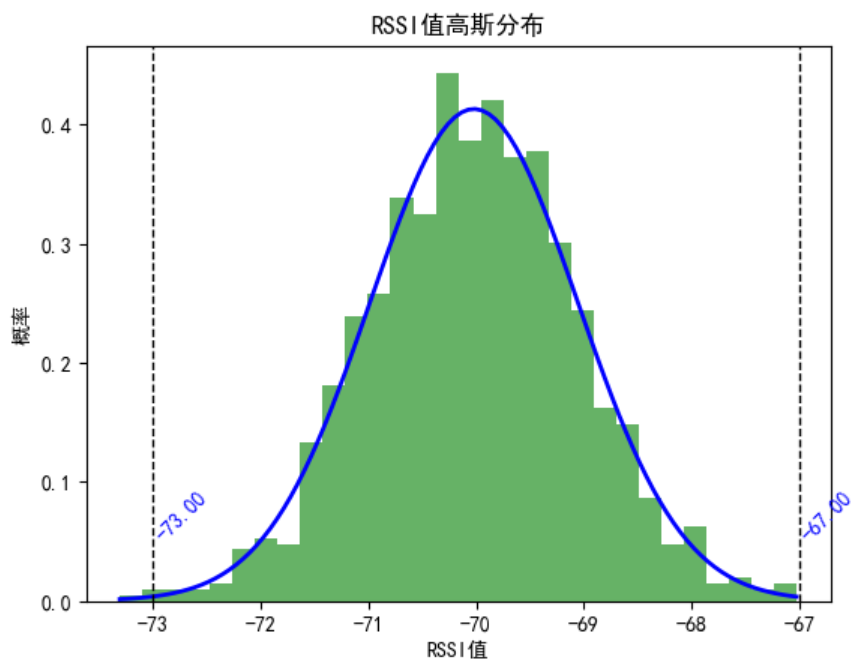
\includegraphics[width=0.7\linewidth]{figures/4.3}
	\caption{RSSI值高斯分布图}
	\label{fig:RSSI值高斯分布图}
\end{figure}

对于max列表数据,使用PD门限和ED门限,求其通过两个门限的通过率,再进行加权求均值,因为ED门限较高,通过较为困难,且通过后抢占信道概率更大,故本研究将PD门限通过率权重为2/3,ED门限通过率权重为1/3。最终得到一个通过率,公式如下所示:

\begin{equation}
	PD\left( RSSI_{max} \right) =\left\{ \begin{array}{l}
		\begin{matrix}
			0&		RSSI_{max}<PD\\
		\end{matrix}\\
		\begin{matrix}
			1&		RSSI_{max}\ge PD\\
		\end{matrix}\\
	\end{array} \right. 
\end{equation}

\begin{equation}
	ED\left( RSSI_{max} \right) =\left\{ \begin{array}{l}
		\begin{matrix}
			0&		RSSI_{max}<ED\\
		\end{matrix}\\
		\begin{matrix}
			1&		RSSI_{max}\ge ED\\
		\end{matrix}\\
	\end{array} \right. 
\end{equation}

\begin{equation}
	Rate_{max}\left( RSSI_{max} \right) =\frac{1}{n}\sum{\left( Wt_{PD}\times PD\left( RSSI_{max}i \right) +Wt_{ED}\times ED\left( RSSI_{max}i \right) \right)}
\end{equation}
\\
最终将数组高维数据降维成一个数。而对于mean列表,以同样的道理,对其使用NAV门限进行计算其通过率,公式如下所示。

\begin{equation}
	NAV\left( RSSI_{mean} \right) =\left\{ \begin{array}{l}
		\begin{matrix}
			0&		RSSI_{mean}<NAV\\
		\end{matrix}\\
		\begin{matrix}
			1&		RSSI_{mean}\ge NAV\\
		\end{matrix}\\
	\end{array} \right. 
\end{equation}

\begin{equation}
	Rate_{mean}\left( RSSI_{mean} \right) =\frac{1}{n}\sum{\left( NAV\left( RSSI_{mean}\_i \right) \right)}
\end{equation}

\subsubsection{传输协议类型数据处理策略}

一次传输过程,由于 TCP 协议头至少为 20byte,UDP 协议头至少为 8byte,所以使用 TCF协议将多花费 20byte,UDP 协议将多花费 8byte。在本题中,无论 UDP 还是 TCP 协议考虑的都是 unicast 模式进行点对点传输数据,每一次传输都需要加上IP协议头且接收节点都会回复 ACK 确认帧,故考虑将数据中的TCP和UDP类别分别替换为20和8,单位为byte,即用协议头花销替代协议类型数据,以达到量化TCP和UDP类别差异。

\subsubsection{分离信号噪声}

在模型准备阶段,本研究已经介绍了如何区分来自不同节点的RSSI信号和噪声。因此,在信号预处理的最后阶段,首先需要对接收自所有节点的RSSI信息进行分离,以区分信号和噪声。在本研究中,信号数据仅存在于上下级节点间的传输中,而接收自其他节点的信息则被视为噪声。
在2AP的情况下,AP仅将与其下级节点STA之间的RSSI数据视为可靠信号,其他节点的RSSI数据则被视为噪声。STA也遵循相同的规则。这一规则同样适用于3AP的情况。

首先对RSSI指标进行优化,在2个AP作用场景中,每两行数据表示在同一次传输数据过程中发送端与接收端相关特征,其中含有多个RSSI相关特征,但对于每一行本身的端口来说,划分为指向性端口对他本身的传输信号RSSI与其他端口对他的干扰信号RSSI,由于是发送端、接收端轮流排列,则导致这一列RSSI中接收到的信息为其他发送端产生的干扰、向本接收端发送的信号轮流排列,而在与之对应的另一列RSSI中,则与之完全相反,呈现出来某一行前后对应的两列数据一个为信号RSSI,一个为其他发送端产生的干扰,为了增加数据特征的表现性与特征显著性,将对应的混乱的两列转化为信号RSSI列和干扰RSSI列。
